\item \textbf{{[}ALVL/9597/2013/P2/Q2{]} }

Examination centres receive examination results for their candidates
as a printed report. The report lists the candidates in order based
on their Index Number. For each candidate their results occupy one
row of the report. Each row displays the results for all subjects
that the candidate sat in the examination.
\begin{center}
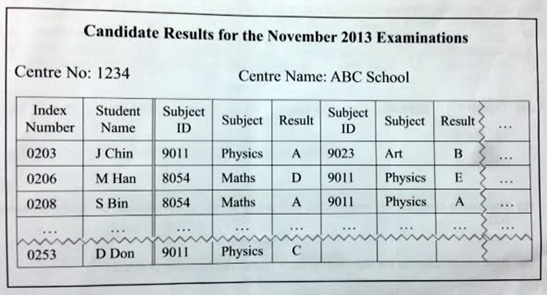
\includegraphics[width=0.5\paperwidth]{C:/Users/Admin/Desktop/Github/question_bank/LyX/static/img/9597-ALVL-2013-P2-Q2-1}
\par\end{center}

Candidates can only take examinations at one centre in a particular
session.

Currently the candidate results for each centre are stored in a separate
file. The software that produces the above report is written in a
programming language.
\begin{enumerate}
\item Describe, using an example, why this file has data redundancy.\hfill{}
{[}2{]}
\item An extra field is added to the file, but the report will not include
this new field. 

Describe the problem that will arise. \hfill{}{[}3{]}
\end{enumerate}
A normalised database solution to this problem is designed, which
has a number of tables.
\begin{enumerate}
\item[(c)]  Draw an E-R diagram that shows these tables and the relationships
between them.\hfill{} {[}5{]}
\item[(d)]  When the data are stored in a database, privacy is of great concern.

Explain why.\hfill{} {[}2{]}
\end{enumerate}